\documentclass[
11pt, % The default document font size, options: 10pt, 11pt, 12pt
%codirector, % Uncomment to add a codirector to the title page
]{charter} 




% El títulos de la memoria, se usa en la carátula y se puede usar el cualquier lugar del documento con el comando \ttitle
\titulo{Solución IoT para robot de exploración ambiental de datos críticos con almacenamiento en blockchain} 

% Nombre del posgrado, se usa en la carátula y se puede usar el cualquier lugar del documento con el comando \degreename
\posgrado{Carrera de Especialización en Internet de las Cosas} 
%\posgrado{Carrera de Especialización en Internet de las Cosas} 
%\posgrado{Carrera de Especialización en Intelegencia Artificial}
%\posgrado{Maestría en Sistemas Embebidos} 
%\posgrado{Maestría en Internet de las cosas}

% Tu nombre, se puede usar el cualquier lugar del documento con el comando \authorname
\autor{Ing. Gonzalo F. Carreño} 

% El nombre del director y co-director, se puede usar el cualquier lugar del documento con el comando \supname y \cosupname y \pertesupname y \pertecosupname
\director{Esp. Ing. Sergio Alberino}
\pertenenciaDirector{UTN.BA} 
% FIXME:NO IMPLEMENTADO EL CODIRECTOR ni su pertenencia
%\codirector{CODIRECTOR} % para que aparezca en la portada se debe descomentar la opción codirector en el documentclass
%\pertenenciaCoDirector{FIUBA}

% Nombre del cliente, quien va a aprobar los resultados del proyecto, se puede usar con el comando \clientename y \empclientename
\cliente{Esp. Lic. Mariano Landini}
\empresaCliente{FCE UBA - Cliente}

% Nombre y pertenencia de los jurados, se pueden usar el cualquier lugar del documento con el comando \jurunoname, \jurdosname y \jurtresname y \perteunoname, \pertedosname y \pertetresname.
\juradoUno{Nombre y Apellido (1)}
\pertenenciaJurUno{pertenencia (1)} 
\juradoDos{Nombre y Apellido (2)}
\pertenenciaJurDos{pertenencia (2)}
\juradoTres{Nombre y Apellido (3)}
\pertenenciaJurTres{pertenencia (3)}
 
\fechaINICIO{1 de julio de 2024}		%Fecha de inicio de la cursada de GdP \fechaInicioName
\fechaFINALPlan{1 de junio de 2025} 	%Fecha de final de cursada de GdP
\fechaFINALTrabajo{20 de octubre de 2025}	%Fecha de defensa pública del trabajo final


\begin{document}

\maketitle
\thispagestyle{empty}
\pagebreak


\thispagestyle{empty}
{\setlength{\parskip}{0pt}
\tableofcontents{}
}
\pagebreak


\section*{Registros de cambios}
\label{sec:registro}


\begin{table}[ht]
\label{tab:registro}
\centering
\begin{tabularx}{\linewidth}{@{}|c|X|c|@{}}
\hline
\rowcolor[HTML]{C0C0C0} 
Revisión & \multicolumn{1}{c|}{\cellcolor[HTML]{C0C0C0}Detalles de los cambios realizados} & Fecha      \\ \hline
0      & Creación del documento.                                 &\fechaInicioName \\ \hline


\end{tabularx}
\end{table}

\pagebreak



\section*{Acta de constitución del proyecto}
\label{sec:acta}

\begin{flushright}
Buenos Aires, \fechaInicioName
\end{flushright}

\vspace{2cm}

Por medio de la presente se acuerda con el \authorname\hspace{1px} que su Trabajo Final de la \degreename\hspace{1px} se titulará ``\ttitle'', consistirá en \textcolor{black}{la implementación de un sistema embebido de robot de exploracion ambiental conectado a un sistema back-end en la nube publica capaz de persistir los datos en una red blockhain}, y tendrá un presupuesto preliminar estimado de \textcolor{black}{\$ 108} dólares estadounidenses y \textcolor{black}{721} horas de trabajo, con fecha de inicio \fechaInicioName\hspace{1px} y fecha de presentación pública estimada \fechaFinalName.

Se adjunta a esta acta la planificación inicial.

\vfill

% Esta parte se construye sola con la información que hayan cargado en el preámbulo del documento y no debe modificarla
\begin{table}[ht]
\centering
\begin{tabular}{ccc}
\begin{tabular}[c]{@{}c@{}}Dr. Ing. Ariel Lutenberg \\ Director posgrado FIUBA\end{tabular} & \hspace{2cm} & \begin{tabular}[c]{@{}c@{}}\clientename \\ \empclientename \end{tabular} \vspace{2.5cm} \\ 
\multicolumn{3}{c}{\begin{tabular}[c]{@{}c@{}} \supname \\ Director del Trabajo Final\end{tabular}} \vspace{2.5cm} \\
%\begin{tabular}[c]{@{}c@{}}\jurunoname \\ Jurado del Trabajo Final\end{tabular}     &  & \begin{tabular}[c]{@{}c@{}}\jurdosname\\ Jurado del Trabajo Final\end{tabular}  \vspace{2.5cm}  \\
%\multicolumn{3}{c}{\begin{tabular}[c]{@{}c@{}} \jurtresname\\ Jurado del Trabajo Final\end{tabular}} \vspace{.5cm}                                                                     
\end{tabular}
\end{table}




\section{1. Descripción técnica-conceptual del proyecto a realizar}
\label{sec:descripcion}

\begin{consigna}{black} % El bloque "consigna" se usa para poner texto en rojo y dar una pequeña ayuda sobre cómo completar la sección. En cada entrega parcial deben eliminar los comandos begin y end del bloque consigna de las secciones que hayan completado.
El presente proyecto es un emprendimiento personal que busca integrar el dispositivo robótico de exploración ambiental controlable a distancia desarrollado en el marco de la carrera de especializacion en sistemas embebidos con un backend para el analisis y explotacion de datos en la nube publica y una red blockchain para el almacenamiento inmutable de datos criticos.

\textit{\textbf{Estado del arte:}}
Los robots exploradores son los dispositivos robotizados que han sido creados con el fin de reconocer y explorar un lugar o terreno siendo capaces de moverse de forma autónoma o controlados por personas a control remoto. Su objetivo es evitar poner en riesgo la vida de los humanos, ya sea debido a que el lugar es inaccesible o porque se encuentra en una zona contaminada.
Algunos de los tipos de robots exploradores más conocidos son los espaciales, de minas, de rescate en catástrofes, de tuberías, acuáticos y/o submarinos, y de suelos.

Estos dispositivos, forman parte de una solución arquitectónica IoT más amplia, cumpliendo el rol de nodos “edge”.  Una vez implementados y funcionando envían lecturas del reconocimiento y operaciones realizadas a sistemas de procesamiento y almacenamiento de datos que conforman el backend, generalmente en la nube, desde donde se puede visualizar los resultados obtenidos, sus métricas derivadas, realizar trazabilidad de las operaciones así como almacenar y gobernar los datos generados. 

En situaciones en las que el robot es utilizado para explorar y monitorear un área ambientalmente sensible, como una reserva natural o un sitio afectado por un desastre ecológico y su misión es recopilar datos críticos -como niveles de contaminación, temperatura, humedad, y calidad del aire- es de gran importancia almacenar estas mediciones de una forma en la que se pueda asegurar la integridad y transparencia de los datos, como por ejemplo, en una cadena de bloques (blockchain).

Una arquitectura blockchain se basa en el procesamiento y almacenamiento de transacciones agrupadas en bloques encadenados e inmutables de forma distribuida entre los nodos de una red en lo que se conoce como un distributed ledger. De esta manera se puede asegurar integridad de los datos ya que los registros generados no se pueden modificar una vez creados. Además, como la red es accesible entre los actores intervinientes en el caso de uso -pudiendo ser pública o privada y con o sin permisos-, se puede garantizar la transparencia de los datos.
La mayoría de las redes blockchain constan de la tecnología para la implementación de código backend ejecutable en la red, que aunque su nombre puede cambiar dependiendo de la red en la cual se implementan, usualmente se los conoce como Smart Contracts. La ejecución de estos componentes es realizada por los nodos de la red en el proceso que se conoce como minería, y como tal es una actividad que requiere el pago de un fee conocido como gas medido en diferentes unidades dependiendo de la red y normalmente pagable desde una cuenta nominada en el token de la red asociada a la aplicación o propietario de los smart contracts. 
La  forma de interactuar con los smart contracts en un caso de uso interactivo desde afuera de la red, se realiza a través de otro componente conocido como dApps (de-centralized applications) que haciendo uso de ciertas librerías de Web3 invocan a estos para almacenar y obtener datos en y desde el ledger.

En el siguiente diagrama se puede apreciar una posible arquitectura del sistema final.



\begin{center}
   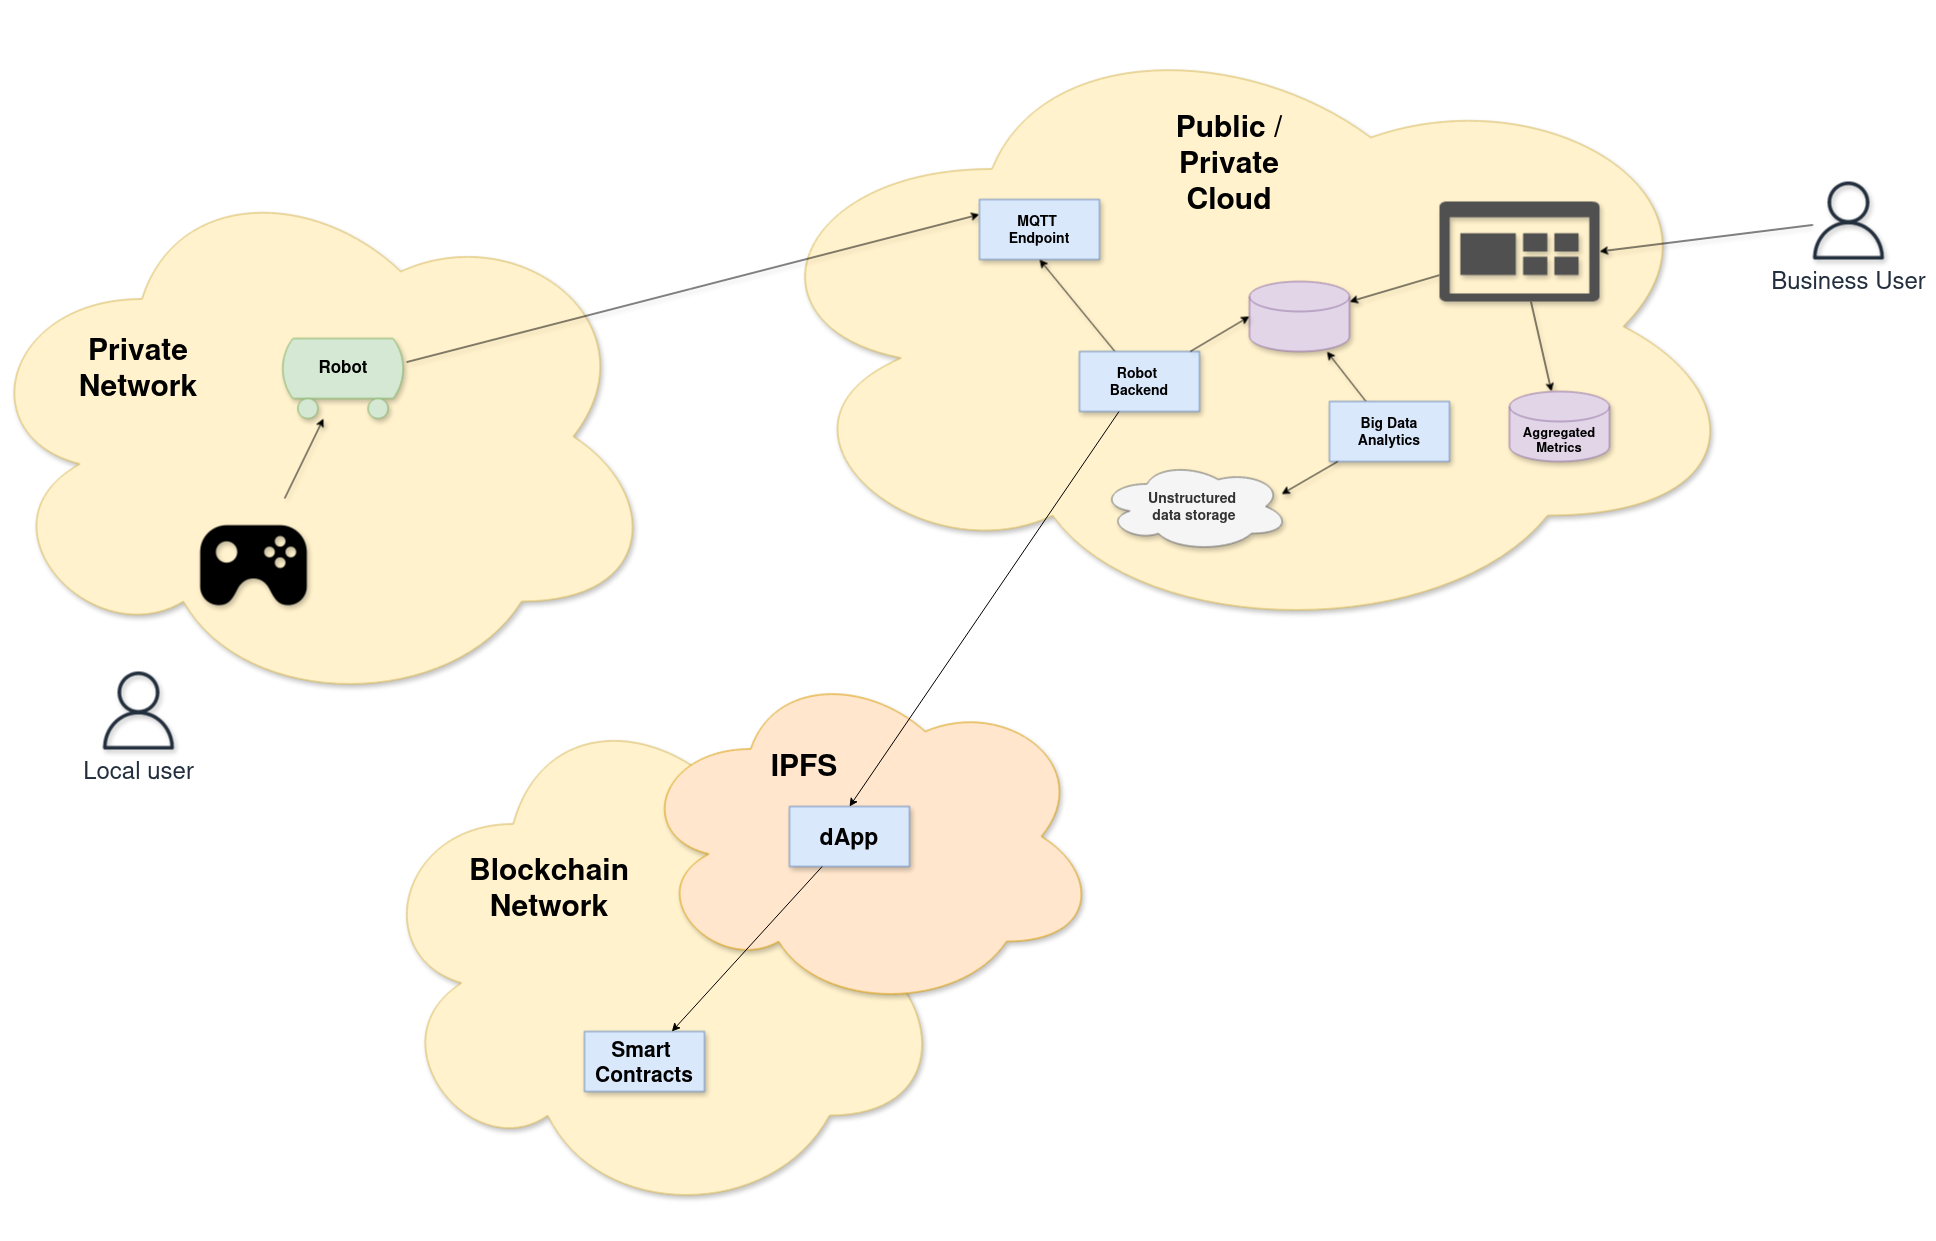
\includegraphics[scale=0.15]{Figuras/IoTProject-Page-1.drawio}
   \captionof{figure}{Arquitectura del sistema}
   \label{fig:esp32}
\end{center}




El hardware utilizado para la solución de IoT propuesta es un robot de exploración ambiental de control inalámbrico, desarrollado en la Carrera de Especialización en Sistemas Embebidos de la Universidad de Buenos Aires. En la siguiente imagen puede apreciarse una fotografía del mismo.

\begin{center}
   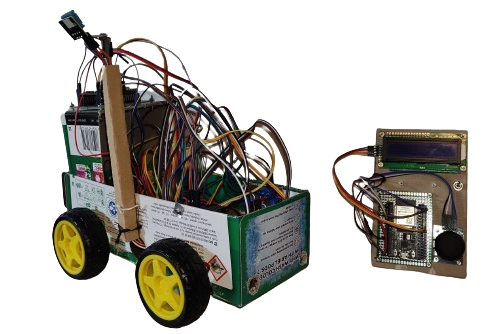
\includegraphics[scale=0.5]{Figuras/Robot_y_Joystick_1}
   \captionof{figure}{Arquitectura del sistema}
   \label{fig:esp32}
\end{center}




\vspace{25px}


\end{consigna}

\section{2. Identificación y análisis de los interesados}
\label{sec:interesados}
\begin{consigna}{black} % este comando se debe borrar para la entrega, junto con la contraparte \end{consigna}{red} 
A continuación se enumeran los diferentes roles e individuos que participarán en el proyecto.
\begin{table}[ht]
%\caption{Identificación de los interesados}
%\label{tab:interesados}
\begin{tabularx}{\linewidth}{@{}|l|l|X|l|@{}}
\hline
\rowcolor[HTML]{C0C0C0} 
Rol           & Nombre y Apellido & Organización 	& Puesto 	\\ \hline

Cliente       & \clientename      &\empclientename	&  -      	\\ \hline
Responsable   & \authorname       & UTN.BA        	& Alumno 	\\ \hline
Orientador    & \supname	      & \pertesupname 	& Director Trabajo final \\ \hline
\end{tabularx}
\end{table}


\end{consigna} % este comando se debe borrar para la entrega, junto con la contraparte \begin{consigna}{red}



\section{3. Propósito del proyecto}
\label{sec:proposito}

\begin{consigna}{black}
El propósito de este proyecto es desarrollar una solución IoT para un robot de exploración ambiental para casos de uso de datos críticos en los que sea necesario contar con almacenamiento inmutable y transparente para todas las partes en una arquitectura blockchain 
Por otra parte, se pretende volcar en un desarrollo concreto y de aplicación industrial los conocimientos adquiridos durante la cursada de la Maestria en Internet de las Cosas.

\end{consigna}

\section{4. Alcance del proyecto}
\label{sec:alcance}

\begin{consigna}{black}
Contando con el hardware mencionado anteriormente que auspicia de componente edge en una arquitectura IoT, se propone la implementación de la plataforma tecnológica que alcanza:

\begin{itemize}
	\item La publicación del endpoint MQTT para la recepción de los datos enviados por el robot.
	\item La adaptación del sistema embebido del robot de exploración ambiental para la conexión segura con el backend vía MQTT.
	\item La arquitectura e implementación de los sistemas backend y el modelo de datos necesario para el almacenamiento de las mediciones enviadas por el robot.
	\item La arquitectura, implementación y despliegue de la dApp (de-centralized application) y Smart Contracts necesarios para el almacenamiento de las mediciones en una red Blockchain (a definir).
	\item La definición de métricas agregadas de valor y posterior arquitectura e implementación de los sistemas analíticos para procesar de forma batch y/o real-time (dependiendo de las métricas a definir) los datos enviados utilizando herramientas de procesamiento paralelo basadas en big data.
	\item La implementación de la interfaz gráfica para poder visualizar los datos enviados y analíticas calculadas.

\end{itemize}


\end{consigna}


\section{5. Supuestos del proyecto}
\label{sec:supuestos}

\begin{consigna}{black}
Para el desarrollo del presente proyecto se supone que: 

\begin{itemize}
	\item será posible tener acceso a redes de desarrollo y testing de forma gratuita mediante la obtencion de Faucets,
	\item será posible experimentar, desarrollar y hacer testing del backend cloud con el presupuesto estimado,
	\item arquitectonicamente resultará viable implementar la solucion propuesta,
	\item se dispondrá del conjunto de librerías, drivers y APIs de bajo nivel para el desarrollo de las funcionalidades planteadas en el alcance sin ser necesario el desarrollo de drivers y dichos componentes de bajo nivel. Ademas, tanto estos componentes de software como los open source de la comunidad de software libre utilizados durante el desarrollo del producto, se encontrará estable para que su integración en el proyecto no resulte en desvíos,	
	\item tanto el prototipado de los componentes de software del sistema embebido como el ensamblado de los componentes de hardware del dispositivo no producirán desvíos considerables en el plan,
	\item no habrá desvíos no contemplados en el plan que impidan o demoren entregas en el proyecto,
	\item el comité académico encargado de la corrección tendrá disponibilidad para realizar la evaluación en las fechas planificadas de entrega,
	\item el director asignado tendrá la disponibilidad de tiempo para darle seguimiento al proyecto,
	\item el alumno contará con una disponibilidad de entre 3 y 5 horas diarias (incluyendo fines de semana) para el desarrollo del proyecto en el tiempo convenido,
	\item los materiales, componentes, software de terceros y servicios cloud utilizados funcionaran de forma óptima y de acuerdo a lo esperado,
	\item el robot desarrollado seguira funcionando de forma estable sin ser necesario su ajuste, reparacion o modificacion a nivel hardware o sistema base (fuera de lo planificado para la integracion con MQTT),
	\item los recursos no directamente relacionados con el desarrollo del proyecto, pero utilizados durante el mismo, funcionaran adecuadamente y en caso de falta de suministro (por ejemplo el servicio de internet) o averia (por ejemplo en el caso de la computadora utilizada) la resolucion sera expeditiva no suponiendo un desvio en el plan,
	\item no sucederan nuevos eventos de impacto global (pandemia, guerras, etc) durante el desarrollo del proyecto que impliquen una demora o imposibilidad en la entrega.
\end{itemize}


\end{consigna}

\section{6. Requerimientos}
\label{sec:requerimientos}
\begin{consigna}{black}
A continuación se listan los requerimientos del producto:

...

\end{consigna}

\section{7. Historias de usuarios (\textit{Product backlog})}
\label{sec:backlog}

\begin{consigna}{black}
A continuacion se listan las historias de usuario. La ponderación de \textit{story points} se realiza considerando 1 punto = 1 hora:

...
\end{consigna}



\section{8. Entregables principales del proyecto}
\label{sec:entregables}
\begin{consigna}{black}
Los entregables del proyecto son:

...
\end{consigna}

\section{9. Desglose del trabajo en tareas}
\label{sec:wbs}

\begin{consigna}{black}
El conjunto de actividades y tareas que se realizarán durante el proyecto son:


\end{consigna}

\section{10. Diagrama de Activity On Node}
\label{sec:AoN}

\begin{consigna}{black}
A continuación se detalla la lista de actividades que se realizarán durante el proyecto. Los tiempos están expresados en días, y como se considera una dedicación de 4 horas diarias (incluyendo fines de semana). 

\begin{table}[ht]
%\caption{Identificación de los interesados}
%\label{tab:interesados}
\begin{tabularx}{\linewidth}{@{}|l|X|l|l|l|@{}}
\hline
\rowcolor[HTML]{C0C0C0} 
Id	& Tarea           									& Duración 			& Dependencia	& Predecesora 	\\ \hline
1	& Gestión del proyecto 								& -		& -				&  - 		\\ \hline
2	& Adquisición de materiales 						& -	& -				&  -      		\\ \hline
3	& Investigación y prototipado						& -		& -				&  -      		\\ \hline
4	& Set-up integración continua (opcional)			& -   	& -        		&  -			\\ \hline
5	& Diseño y desarrollo de funcionalidades    		& -		& -			 	& -			\\ \hline
6	& Testing								    		& -		& -				& -			\\ \hline
7	& Ensamblado del hardware				    		& -		& -				& -				\\ \hline
8	& Funcionalidades extras (opcional)					& -		& -				& - 			\\ \hline
9	& Documentación    									& -		& -			 	& -				\\ \hline

\end{tabularx}
\end{table}

\end{consigna}


\section{11. Diagrama de Gantt}
\label{sec:gantt}

\begin{consigna}{black}


\end{consigna}

\section{12. Presupuesto detallado del proyecto}
\label{sec:presupuesto}

\begin{consigna}{black}
El siguiente cuadro presenta los costos en dólares estadounidenses estimados para el proyecto:

\end{consigna}

\begin{table}[htpb]
\centering
\begin{tabularx}{\linewidth}{@{}|X|c|r|r|@{}}
\hline
\rowcolor[HTML]{C0C0C0} 
\multicolumn{4}{|c|}{\cellcolor[HTML]{C0C0C0}COSTOS DIRECTOS} \\ \hline
\rowcolor[HTML]{C0C0C0} 
Descripción &
  \multicolumn{1}{c|}{\cellcolor[HTML]{C0C0C0}Cantidad} &
  \multicolumn{1}{c|}{\cellcolor[HTML]{C0C0C0}Valor unitario} &
  \multicolumn{1}{c|}{\cellcolor[HTML]{C0C0C0}Valor total} \\ \hline
 - & 
  \multicolumn{1}{c|}{1} &
  \multicolumn{1}{c|}{\$ 0,00} &
  \multicolumn{1}{c|}{\$ 0,00} \\ \hline
 - &
  \multicolumn{1}{c|}{1} &
  \multicolumn{1}{c|}{\$ 0,00} &
  \multicolumn{1}{c|}{\$ 0,00} \\ \hline
 - &
  \multicolumn{1}{c|}{1} &
  \multicolumn{1}{c|}{\$ 0,00} &
  \multicolumn{1}{c|}{\$ 0,00} \\ \hline
 - &
  \multicolumn{1}{c|}{1} &
  \multicolumn{1}{c|}{\$ 0,00} &
  \multicolumn{1}{c|}{\$ 0,00} \\ \hline
 - &
  \multicolumn{1}{c|}{1} &
  \multicolumn{1}{c|}{\$ 0,00} &
  \multicolumn{1}{c|}{\$ 0,00} \\ \hline
 - &
  \multicolumn{1}{c|}{1} &
  \multicolumn{1}{c|}{\$ 0,00} &
  \multicolumn{1}{c|}{\$ 0,00} \\ \hline
 - &
  \multicolumn{1}{c|}{1} &
  \multicolumn{1}{c|}{\$ 0,00} &
  \multicolumn{1}{c|}{\$ 0,00} \\ \hline
 - &
  \multicolumn{1}{c|}{1} &
  \multicolumn{1}{c|}{\$ 0,00} &
  \multicolumn{1}{c|}{\$ 0,00} \\ \hline
 - &
  \multicolumn{1}{c|}{1} &
  \multicolumn{1}{c|}{\$ 0,00} &
  \multicolumn{1}{c|}{\$ 0,00} \\ \hline
 - &
  \multicolumn{1}{c|}{1} &
  \multicolumn{1}{c|}{\$ 0,00} &
  \multicolumn{1}{c|}{\$ 0,00} \\ \hline
\rowcolor[HTML]{C0C0C0} 
\multicolumn{3}{|c|}{TOTAL} &
  \multicolumn{1}{c|}{\$ 0,00} \\ \hline
\end{tabularx}%
\end{table}


\section{13. Gestión de riesgos}
\label{sec:riesgos}
\begin{consigna}{black}

\end{consigna}


\section{14. Gestión de la calidad}
\label{sec:calidad}
\begin{consigna}{black}

\end{consigna}

\section{15. Procesos de cierre}   
\label{sec:cierre}
\begin{consigna}{black}

\end{consigna}




\end{document}
